\cleardoublepage

\section{引言}

\subsection{研究意义}
近年来,神经网络的成功应用促进了模式识别和数据挖掘等领域的研究。许多机器学习任务
,如目标检测[1],机器翻译[2]和语音识别[3],曾经非常依赖人工来提取特征信息,现在可
以通过各种端到端深度学习范式来完成,如卷积神经网络[4],循环神经网络[5]和自动编码
器[6]。深度学习在很多领域的成功归功于快速发展的计算资源(GPU)、大量可用于训练的
数据、以及从欧几里得数据(图像、文本、视频)中提取特征的能力。以图像数据为例,我们
可以将欧几里得空间中的图像表示为规则网络,卷积神经网络能够利用图像数据的平移不变性、
局部连通性和合成性来提取特征,因此卷积神经网络可以提取能够应用于整个数据集的局部有效
特征信息。

虽然深度学习可以有效地捕捉欧几里得数据的特征,但越来越多的应用程序将数据表示为图数据。
对于一些从非欧几里得域生成的数据,如社会网络、经济网络、信息网络、流行病学网络、传感
器网络中的数据,人们处理和分析他们的需求正在日益增长。
具体来说,在电子商务中,基于图结构的深度学习模型可以利用用户和产品之间的交互来做出高度准确
的推荐。在化学中,分子被建模为图,它们的生物活性需要被识别以用于药物发明。在引
文网络中,论文是通过引文相互联系的,它们需要被分成不同的类别。

然而,图数据的复杂性给现有的机器学习算法带来了巨大的挑战,这主要有以下原因。首先,由于图
可能是不规则的,一个图可能有一个可变大小的无序节点;其次,一个图的节点可能有不同数量的
邻居,导致一些重要的操作(如卷积运算)很容易在图像域计算,但很难应用到图域;此外,现有机器
学习算法的一个核心假设是实例是相互独立的,这个假设不再适用于图数据,因为每个
实例通过各种类型的连接(如引用、交互)与其他实例相关联。

\subsection{研究现状}
为了处理和利用图数据,在图信号处理领域,有学者提出了图信号的高效表示方法,并且建立
了关于图的移位、滤波、卷积、傅立叶变换、频谱分解等一系列概念[7];此外,有很多研究者
尝试使用图变换算子(GSO)的矩阵多项式[8],来设计可以分析图信号和设计的图滤波器,这些
图滤波器可以被用于信号预测、信号压缩、分类任务等应用。

在深度学习领域,也正在有越来越多关于图神经网络(GNNs)的研究。学者们先
后提出了递归图神经网络(RecGNNs)、图卷积神经网络(ConvGNNs)、图自编码器
(GAEs)、时空图神经网络(STGNNs)等神经网络结构,见图\ref{1-1}。其中,ConvGNNs 汲取了图信
号处理领域的思想,将卷积运算从网格数据推广到图数据。目前,ConvGNNs 已经
在节点级分类的半监督学习、图级分类的监督学习、用于图嵌入的无监督学习等任务里取得
了前所未有的效果;并且在其他复杂的GNNs 模型中,ConvGNNs 也发挥着核心作
用。

\begin{figure}[ht]
    \centering
    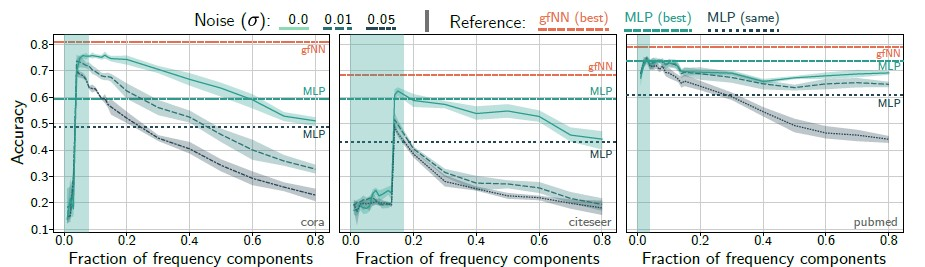
\includegraphics[width=12cm]{introduction/1.jpg}
    \caption{\label{1-1}图神经网络(GNNs)的分类}
\end{figure}

\begin{itemize}
    \item \textbf{递归图神经网络(RecGNNs)} \quad
    RecGNNs大多是图神经网络的先驱作品。RecGNNs的目的是通过循环神经网络结构,来学习节点
    表示。他们假设图中的一个节点不断地与它的邻居交换信息,直到达到一个稳定的均衡。
    RecGNNs在概念上很重要,启发了图卷积神经网络的后续研究,特别是,基于空间的图卷积神经
    网络继承了信息传递的思想[9]。
    
    \item \textbf{图卷积神经网络(ConvGNNs)} \quad
    ConvGNNs将卷积运算从网格数据推广到图数据。其主要思想是通过聚合节点$v$自身的特征$x_{v}$
    和邻居的特征$x_{u}$来生成节点$v$的表示,其中$u\in N(v)$。与RecGNNs不同,ConvGNNs将多个
    图卷积层堆叠起来,提取高级节点表示。在建立许多其他复杂的GNN模型中,ConvGNNs发挥着核心作
    用。如图\ref{1-2}中ConvGNN被用于节点的分类,图\ref{1-3}中ConvGNN被用于图的分类。

    \item \textbf{图自编码器(GAEs)} \quad
    GAEs是一种无监督学习框架,它将节点或图编码成一个潜在的向量空间,并从编码的信息重构图数据。
    该算法用于学习网络嵌入和图生成分布。对于网络嵌入,GAEs通过重构图的邻接矩阵等图结构信息来
    学习潜在节点表示[10],如图\ref{1-4}。对于图的生成,有的方法是一步一步生成图的节点和边,有的
    方法是一次性输出图。

    \item \textbf{时空图神经网络(STGNNs)} \quad
    STGNNs的目的是从时空图中学习隐藏的模式,这在各种应用中变得越来越重要,如交通速度预测,驾驶员操纵
    预测,人类行为识别。STGNNs的核心思想是同时考虑空间依赖和时间依赖。目前的许多方法都是通过图卷
    积来捕获与RNNs或CNNs的空间依赖关系,从而对时间依赖关系进行建模,如图\ref{1-5}。
\end{itemize}

\begin{figure}[htbp]
    \centering
    \begin{minipage}[t]{0.48\textwidth}
    \centering
    \captionsetup{width=5cm}
    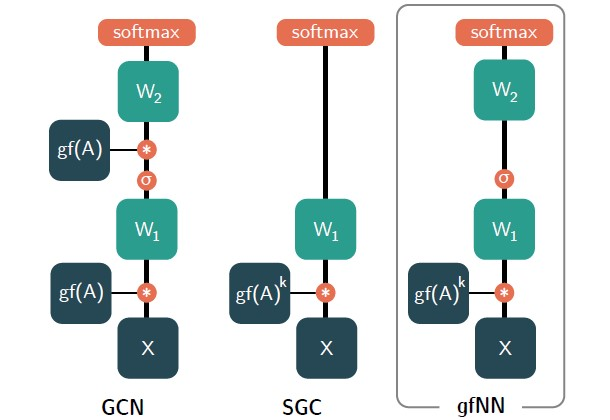
\includegraphics[width=6cm]{introduction/2.jpg}
    \caption{\label{1-2}通过堆叠多层卷积层,来获得邻节点的信息,用于节点的分类}
    \end{minipage}
    \begin{minipage}[t]{0.48\textwidth}
    \centering
    \captionsetup{width=5cm}
    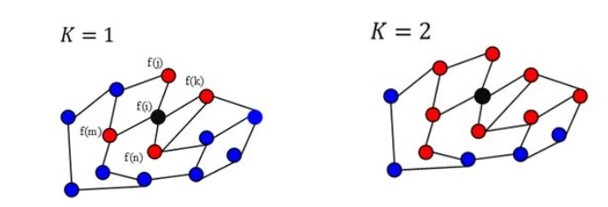
\includegraphics[width=6cm]{introduction/3.jpg}
    \caption{\label{1-3}通过卷积层和池化层,来提取特征信息,并最终用于图的分类}
    \end{minipage}
\end{figure}
\begin{figure}[htbp]
    \centering
    \begin{minipage}[t]{0.48\textwidth}
    \centering
    \captionsetup{width=5cm}
    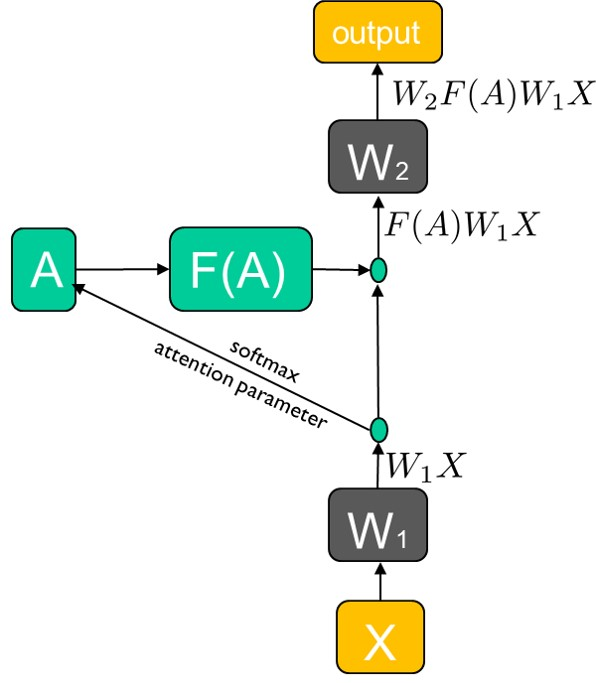
\includegraphics[width=6cm]{introduction/4.jpg}
    \caption{\label{1-4}编码器使用图卷积层得到每个节点的网络嵌入,解码器重构图邻接矩阵}
    \end{minipage}
    \begin{minipage}[t]{0.48\textwidth}
    \centering
    \captionsetup{width=5cm}
    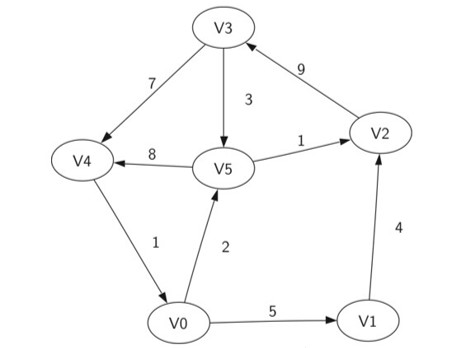
\includegraphics[width=6cm]{introduction/5.jpg}
    \caption{\label{1-5}图卷积层对$A$和$X^(t)$进行操作以捕获空间特性,而1D-CNN层沿时间轴在$X$上滑动以捕获时间特性}
    \end{minipage}
\end{figure}

\subsection{主要贡献}
我们工作的主要贡献总结如下:
\begin{itemize}
    \item \textbf{回顾图卷积神经网络} \quad
    我们从基于频谱理论和基于空间理论的设计角度,讨论了图卷积神经网络设计的基本理论和方法,
    并且对代表性的模型进行了详细的叙述,进一步对比了这两种设计方法的优劣和应用场景。

    \item \textbf{验证图信号处理的理论} \quad
    图信号处理领域的研究结果表明:对于图数据而言,图卷积神经网络的效果类似于“低通滤波器”。
    此结论已经在基于频谱理论的神经网络设计上得到了验证和应用,我们则进一步将这个结论应用到基于空间
    理论的图卷积神经网络设计上,并且验证了此结论的有效性。

    \item \textbf{设计新的图卷积神经网络} \quad
    我们从“图卷积神经网络能够等效于低通滤波器”这一结论出发,将频谱理论和空间理论的设计方法相结合,设计
    了一种具有高效率和强表达能力的新图卷积神经网络(our GAT),并且在Cora、Citeseer和Pubmed数据集上
    测试了我们新网络。
\end{itemize}

\subsection{论文思路}
这篇毕业论文的行文思路如下。第2节,作为图卷神经网络设计的理论基础,我们分别介绍了基于频谱理论和基于空间理论
的设计思路,并且分析了它们的区别和优劣;第3节,我们从图信号处理领域的结论出发,阐述了我们
的设计思路,并且详述了我们所提出的新图卷积神经网络(our GAT)的结构;第4节,我们在Cora等数据集上测试了我们的新网络,
并且做了一系列相关实验,验证了其高效率和强大的表达能力;第5节,我们讨论和展望未来的潜在研究方向。